% The packages used here are just a sample. You may need others, and may not need some of these. It doesn't hurt to leave them in, unless they start to conflict with other packages you've added. Chapter 2 has example code for equations, figures, tables, citations, abbreviations, etc. If there are sections labeled 'optional' that you don't want, just comment them out. -jg

\documentclass[reqno,12pt,oneside]{report} % right-side equation numbering, 12 point font, print one-sided 
%\documentclass[reqno,12pt,twoside,openright]{report} % right-side equation numbering, 12 point font, print two-sided, Chapters start on odd pages. Rackham only accepts one-sided, so this is for personal printings.

\usepackage{rac}         % Use Rackham thesis style file
\usepackage{aas_macros}  % To allow the reading of ADS journal references in the bibliography
\usepackage[intlimits]{amsmath} % Puts the limits of integrals on top and bottom
\usepackage{amsxtra}     % Use various AMS packages
\usepackage{amsthm}
\usepackage{amssymb}
\usepackage{amsmath}
\usepackage{bm}% bold math
\usepackage{amsfonts}
\usepackage{graphicx}    % Add some packages for figures. Read epslatex.pdf on ctan.tug.org
\usepackage{rotating}
\usepackage{color}
\usepackage{epsfig}
\usepackage{subfigure}   % To make subfigures. Read subfigure.pdf on ctan.tug.org
\usepackage{verbatim}
\usepackage{natbib}      % Allows you to use BibTeX
\usepackage[printonlyused]{acronym} % For the List of Abbreviations. Read acronym.pdf on ctan.tug.org
\usepackage{setspace}    % Allows you to specify the line spacing
\doublespacing           % \onehalfspacing for 1.5 spacing, \doublespacing for 2.0 spacing.
\newcommand{\sun}{\ensuremath{\odot}} % sun symbol is \sun
\newcommand{\angstrom}{\mbox{\normalfont\AA}} %for angstrom symbol
%%%%%%%%%%%%%%%%%%%%%%%%%%%%%%%%%%%%%%%%%%%%%%%%%%%%%%%%%%%%%%%%%%%%%%%%%%%%%%%

% Various theorem environments. All of the following have the same numbering
% system as theorem.

\theoremstyle{plain}
\newtheorem{theorem}{Theorem}
\newtheorem{prop}[theorem]{Proposition}
\newtheorem{corollary}[theorem]{Corollary}
\newtheorem{lemma}[theorem]{Lemma}
\newtheorem{question}[theorem]{Question}
\newtheorem{conjecture}[theorem]{Conjecture}
\newtheorem{assumption}[theorem]{Assumption}

\theoremstyle{definition}
\newtheorem{definition}[theorem]{Definition}
\newtheorem{notation}[theorem]{Notation}
\newtheorem{condition}[theorem]{Condition}
\newtheorem{example}[theorem]{Example}
\newtheorem{introduction}[theorem]{Introduction}

\theoremstyle{remark}
\newtheorem{remark}[theorem]{Remark}
%%%%%%%%%%%%%%%%%%%%%%%%%%%%%%%%%%%%%%%%%%%%%%%%%%%%%%%%%%%%%%%%%%%%%%%%%%%%%%%

\numberwithin{theorem}{chapter}     % Numbers theorems "x.y" where x
                                    % is the section number, y is the
                                    % theorem number

%\renewcommand{\thetheorem}{\arabic{chapter}.\arabic{theorem}}

%\makeatletter                      % This sequence of commands will
%\let\c@equation\c@theorem          % incorporate equation numbering
%\makeatother                       % into the theorem numbering scheme

%\renewcommand{\theenumi}{(\roman{enumi})}

%%%%%%%%%%%%%%%%%%%%%%%%%%%%%%%%%%%%%%%%%%%%%%%%%%%%%%%%%%%%%%%%%%%%%%%%%%%%%%

% If printing two-sided, this makes sure that any blank page at the 
% end of a chapter will not have a page number. 
\makeatletter
\def\cleardoublepage{\clearpage\if@twoside \ifodd\c@page\else
\hbox{}
\thispagestyle{empty}
\newpage
\if@twocolumn\hbox{}\newpage\fi\fi\fi}
\makeatother 

%%%%%%%%%%%%%%%%%%%%%%%%%%%%%%%%%%%%%%%%%%%%%%%%%%%%%%%%%%%%%%%%%%%%%%%%%%%%%%

%This command creates a box marked ``To Do'' around text.
%To use type \todo{  insert text here  }.

\newcommand{\todo}[1]{\vspace{5 mm}\par \noindent
\marginpar{\textsc{To Do}}
\framebox{\begin{minipage}[c]{0.95 \textwidth}
\tt\begin{center} #1 \end{center}\end{minipage}}\vspace{5 mm}\par}

%%%%%%%%%%%%%%%%%%%%%%%%%%%%%%%%%%%%%%%%%%%%%%%%%%%%%%%%%%%%%%%%%%%%%%%%%%%%%%%
\DeclareUnicodeCharacter{2212}{-} %WARNING WARNING added by Mingfei
\overfullrule=0pt %WARNING WARNING added by Mingfei

\usepackage[]{graphicx}
\usepackage{lineno}
\usepackage[caption=false]{subfig}

\begin{document}

\bibliographystyle{agu04}    % Set the bibliography style. agu04, plain, alpha, etc. Original Rackham
%\bibliographystyle{alpha}    % Set the bibliography style. agu04, plain, alpha, elsarticle-num-names, etc.

% Title page as required by Rackham dissertation guidelines
\titlepage{Atomistic simulations of thermodynamics and kinetics related to advanced alloy processing}{Mingfei Zhang}{Doctor of Philosophy}
{Materials Science and Engineering}{2020}
{Assistant Professor Liang Qi, Chair\\
 Professor Amit Misra\\
 Associate Professor Emmanouil Kioupakis\\
 Professor Fei Gao}

% Begin the front matter as required by Rackham dissertation guidelines
\initializefrontsections

% Optional Frontispiece
%\frontispiece{\includegraphics[width=6in]{Intro/Happy} Find a cool picture to go here.}

% Optional, but recommended, Copyright page
%\copyrightpage{Your Name}

% Page numbering. If you don't include a frontispiece or copyright page, you'll need to change this for two-sided printing.
\makeatletter
\if@twoside \setcounter{page}{4} \else \setcounter{page}{1} \fi
\makeatother
 
% Optional Dedication page
\dedicationpage{Dedicated to my family.}

% Optional Acknowledgements page
\startacknowledgementspage
I will do the acknowlegement part later...
Prof. Qi, other committee members, MSE department
Yong-Jie, Chaoming, Aditya, Zhucong, 
My friends Ruiming, Dandan, Patrick, Judy,
Nocona, 
Dr. Louis Hector, Jr., Dr. Cheng Zhang, Prof. Jay Guo, Dr. Jing-Yu Lao.
My parents and wife
U-M HPC, stampede2, nersc,
Guardian, GM, NSF-GOALI
\label{Acknowledgements}

% Optional Preface page
%\startprefacepage
%\input{Preface}
%\label{Preface}

% Table of contents, list of figures, etc.
\tableofcontents     % Required
\listoffigures       % Required if there is more than one figure
\listoftables        % Required if there is more than one table
%\listofmaps          % Required if there is more than one map
\listofappendices    % Required if there is more than one appendix
\listofabbreviations % Optional. Abbreviations should be stored in a file named abbr.tex

% Optional in-dissertation Abstract Page
\startabstractpage
{Atomistic simulations of thermodynamics and kinetics related to advanced alloy processing}{Mingfei Zhang}{Chair: Liang Qi}
In my dissertation, the thermodynamic driving forces and kinetics of critical reaction steps during advanced alloy processing are studied systematically by theoretical models and simulation tools at the atomistic scale. These efforts include improving the Ag thin-film quality during sputtering, discovering a build-in corrosion-resistant mechanism for cast Mg alloys, and slowing down cluster nucleation and growth in Al solid solution alloys during natural aging to avoid costly hot stamping procedures. First, the thermodynamic driving force of H adsorption on anion-terminated (000$\overline{1}$) surfaces of pure and doped wurtzite ZnO as dielectric substrates are investigated under varying H surface coverage conditions. Understanding of these H adsorption mechanisms provides a general way to design substrate surfaces with desired binding strengths for the Ag thin-film. Second, \acf{GCMC} simulations are conducted to simulate the deposition "kinetics" of Ag thin film on substrates, which can be constructed based on the structures and properties of H-adsorbed ZnO (000$\overline{1}$) surfaces. The results demonstrate the reason why ZnO is the most suitable substrate for Ag thin film deposition and the mechanism to achieve thinner continuous Ag films by adding "anchor'' sites on the substrate surface. We use first-principles calculations to search for potential dopant elements as good "anchor'' sites on ZnO substrates and other dopants to stabilize the Ag grain boundaries to improve the polycrystalline Ag thin-film during heat treatment. Third, the \acf{HER} as the cathodic reaction on surfaces of the second-phase transition-metal (Fe) particles can speed up the corrosion of cast Mg metals and alloy. Thus, thermodynamic criteria to slow down the HER are used for high-throughput first-principles computations to search alloying elements that can reduce HER rate to achieve build-in corrosion resistance for cast Mg alloys. Our first-principles search goes across the periodic table and discovers six p-block elements that can increase the corrosion resistance for Mg, consistent with the available experimental results. Fourth, \acf{kMC} simulations are performed to study the early transition behavior from a supersaturated solid solution to \acf{GP} zone of Al 7000 series alloys at room temperature (so-called natural aging), which is critical for their thermal-mechanical processing in automobile manufacturing. Our kMC method include a \acf{NN} model trained by thousands of \ac{DFT} calculations to accurately predict vacancy migration barriers in Al-Mg-Zn-based alloys. Besides, advanced modeling approaches like \acf{LRU} cache and \acf{LSKMC} are also implemented to speed up the kMC simulations in order to directly study the natural aging of Al alloys in the realistic time scales.
\label{Abstract}

\startthechapters 
% The individual files for each of the chapters are put here.
% Save each chapter of your thesis to a seperate tex file
% and then use the \input command to include this file in your
% thesis.  For instance you can save a file to "intro.tex" and 
% then type \input{intro}. 

 \chapter{Introduction}
 \label{chap:Intro}
 \newpage
\section{Background}

Humans in all times have never stopped the discovery of innovative alloys. The application of alloying metals allows the metallurgist to customize the properties by combining various properties of metals together and using the metals interactions to provide unique different alloys. Alloying basically provides the opportunity of inventing new materials where the desired properties are the target.

And the history of alloy processing is a history of mankind itself. Metallurgists have been making every effort to test and invent new desired alloys. As the requirements of the quality and combination of different properties of materials become higher, more costly and complicated processing techniques have to be used. The development of materials has always been strongly guided by economic factors. Those techniques and facilities are suitable for high-technology high-profit industries, like semiconductor and aviation manufactures. However, many of those techniques are not affordable to transfer to civil industry products, like architecture glasses, automobile frames, and so on.

For example, thin-film deposition manufacturing is essential for solar panels, electronic and optical devices manufacturers today. Basically, thin-film deposition applies a very thin film of materials of $\sim$nanometers to $\sim$micrometers onto a surface to be coated, or onto a previously deposited layer to form layers. In order to put billions of transistors into a small CPU or build multiple-layer photodiodes, advanced deposition methods, like chemical vapor deposition (CVD), physical vapor deposition (PVD) or atomic layer deposition (ALD), is used. In these methods, ultra-high vacuum status will be reached in the chamber to achieve the highest thin film quality. However, it is impossible to apply those techniques to large scale coating on architectural glasses for low-emissivity or anti-glaring purposes.

Not only 2D materials, but bulk materials also need some expensive ``magic'' to make materials to be easily machined. For example, structural alloys need high specific strength and long product life cycles. They also require a special shape to function properly. The ability to create materials of high yield strength and yet high ductility has been very challenging for a long time. Aluminum alloys can be subjected to costly procedures, such as controlled hot-working, warm stamping, and coupled solutioning-quenching-stamping operations in a narrow time window, followed by artificial aging to achieve precipitate hardening. The procedures described above are widely used in the aerospace industry but not suitable for the automobile industry or other civil industries that need high strength-weight-ratio.

On the other hand, corrosion resistance is another important property for alloys. Usually, the corrosion-resistant coating is used in automobile industries. However, the ability to resist corrosion decreases during serving, especially if small scratches appear. This traditional coating protection alone increases the cost of maintenance.
\section{Outline}

In this work, efforts were made to solve problems related to alloy processing mentioned above. The target is to combine adding a trace amount of element and affordable processing techniques to make materials with relatively high-quality for large-scale commercial applications. Attentions are paid to achieve ultra-thin Ag films under regular vacuum conditions, to increase Mg alloy corrosion resistance, and to increase formability for high strength Al alloys. To achieve these targets, the trace amount of element added to the alloy will either change the thermodynamic driving force or the activation barriers related to kinetics during the processing procedures. Because the amount of alloying elements added is minimal, it is expected that such alloying would not affect the original properties of alloys significantly. The rest of this dissertation is organized as the following.

In Chapter \ref{chap:Methods}, the fundamental principles of the computational methods applied in the present dissertation are discussed in detail, including 1) the background and details for first-principles calculations, 2) the \acf{GCMC} simulations, 3) the \acf{MC} simulations, and 4) deep learning and neural network methods trained by first-principles calculation results to predict the activation barriers of vacancies in multicomponent alloys.

In Chapter \ref{chap:ZnO_H}, the effects of alloying elements on the hydrogen (H) equilibrium coverage on zinc oxide (ZnO) and other similar semiconductor surfaces are investigated systematically. This study can enhance our understanding of the semiconductor substrate conditions for silver (Ag) thin film deposition. The electronic mechanism of H equilibrium coverage on pure ZnO surfaces and those with alloying elements (Na, Mg, Al, Ti, Fe, Pb, Sn, and V) are studied. The simple bond-counting mechanism is proposed to determine and manipulate the equilibrium H adsorption configurations for different alloying surfaces. Besides, the generalization of this mechanism on other different semiconductor polar surfaces with chemical dopant elements are also discussed. 

Follow the previous study of H equilibrium coverage on ZnO surfaces, in Chapter \ref{chap:Ag/ZnO}, atomistic \acf{GCMC} simulations of Ag deposition on ZnO surfaces are performed to investigate the key parameters that control the quality of Ag thin films. First, the possible reasons why the ZnO substrate is appropriate for high-quality (continuous and crystalline states) Ag thin films are proposed. Then, pseudo-atoms are added on the ZnO surfaces as ``anchor'' sites in GCMC simulations to achieve ultra-thin Ag film under regular low vacuum conditions. Following this, first-principles high-throughput calculations are conducted to search suitable ``anchor'' site choices that match the requirements from the above GCMC simulations. Last but not least, efforts are made to search elements than can segregate to Ag grain boundaries (GBs) to stabilize GBs and the thin-film quality during the high-temperature heat treatment processing. So far, first-principle calculation results on GB separations have some discrepancies with the experimental observations, but possible reasons are explained, and a new methodology to resolve this inconsistency is proposed.

In Chapter \ref{chap:Mg_H}, because the \acf{HER} on second-phase transition metal particles is the cathodic reactions of the Galvanic corrosion in Mg alloy, thermodynamic criteria are proposed to slow down the HER rate on surfaces of these particles. Based on these criteria, we perform high-throughput first-principles calculations to search for possible alloy elements that can slow down HER to achieve build-in corrosion resistance for Mg alloys.  Our first-principles computational procedure goes across all metal and semi-metal elements in the periodic table. The results suggest that six promising p-block elements slow down the HER on the surfaces of common Fe impurities from the casting processing. The most effective two elements of them (As and Ge) are in accord with recent experiments. The electronic mechanism to reduce the HER rate on these surfaces is also discussed. Moreover, the generalization ability of this high-throughput computation paradigm is also tested on other precipitates as potential active sites for the cathodic corrosion reaction. 

Chapter \ref{chap:Al/Vac} focuses on the methodology development on simulating the solute clustering kinetics in multicomponent Al alloys quantitatively. To slow down solute clustering at room temperatures (so-called natural aging) after the high-temperature solid-solution treatment is crucial to expand the time window for the mechanical forming of certain high-strength multicomponent Al alloys, such as 7000 series Al-Mg-Zn alloys. Since the clustering is achieved by solute diffusion based on vacancy migration, we first discuss the relationship between vacancy migration barriers and local lattice occupation environments. It is found that the traditional bond counting method fails to predict vacancy migration barriers for the multicomponent systems. Second, a \acf{NN} surrogate model based on the first-principle training data set is introduced to predict the vacancy migration barrier accurately. Third, a \acf{kMC} simulation package based on \ac{NN} model with advanced acceleration methods, such as parallel schema, \acf{LRU} cache, \acf{LSKMC} is introduced to simulate the solute clustering kinetics in multicomponent Al alloys. Last but not least, the visualization and characterization methods of solute clusters in the kMC simulation results are investigated. The information on cluster compositions and structures lays the foundation for the studies of the clustering effects on the strengths and formability of multicomponent Al alloys in the future.

All of the above studies are related to the thermodynamics and kinetics of alloy processing at the atomistic scale. These studies can be understood in an integrated way described as the following. For complex kinetics related to alloy processing, it is more convenient to divide a complicated full reaction path into many elementary reaction steps. Then the efforts are made to investigate the elementary steps, especially those critical rate-determining ones. There are two general types of investigation approaches for these elementary steps. The studies from Chapter \ref{chap:ZnO_H} to Chapter \ref{chap:Mg_H} are performed under the ``quasi-equilibrium'' kinetic approximation, which is based on the assumption that the thermodynamic equilibrium is achieved for most elementary steps except the rate-determining ones. In addition, to further simplify the first-principles calculations, the kinetic barrier of each elementary step is assumed to be not significantly deviated from the maximum thermodynamic driving force. Therefore, only the energy differences ($\Delta E$) between initial and final states of the critical elementary steps will be investigated, and the kinetics of elementary steps will be derived or simulated based on these energy differences (the kinetic barrier $E_a = 0$ if the energy driving force $\Delta E < 0$, otherwise $E_a \sim \Delta E$). On the other hand, only studies in Chapter \ref{chap:Al/Vac} are conducted based on the prediction of the accurate activation barrier and kinetics in every single elementary step. This direct approach is critical for the accurate prediction of kinetics in multicomponent alloy systems, where the shapes of the potential energy landscape are so complex that the simple assumptions on the relations between thermodynamics and kinetics may fail.  Thus, the studies in this thesis provide a comprehensive portrayal to future researchers to choose appropriate methods to investigate the alloying processing at the atomistic scale.

Finally, Chapter \ref{chap:Conc} concludes the thesis and provides some thoughts on future works.


 \chapter{Methods}
 \label{chap:Methods}
 \section{Density Functional Theory}
\label{Chap:Mech:DFT}

In order to investigate interactions between hydrogen atoms and free surfaces of metals or oxides, we need to study their electronic structures. On the other hand, an accurate diffusion barrier energy also relies on a accurate reaction pathway. These can be achieved by first-principles methods. The calculation of interactions between the positively charged nuclei and negatively charged electrons is considered to be a many-body problem combining kinetic energy, interactions between nuclei and electrons, and electron-electron interactions. In principle, a quantum mechanical solution to this many-body problem with $N$ electrons in an external potential $V_{ext}(r)$ generated by the nuclei can be obtained by solving the Schr\"{o}vdinger’s equation. Based on the Born-Oppenheimer approximation, the motion of nuclei and electrons can be considered separately. Besides, $V_{ext}(r)$ can be obtained by calculating the Coulomb interactions between the atomic nuclei and electrons. The time-independent, non-relativistic Schr\"{o}dinger's equation for an N-electrons system can be written as,
\begin{subequations}
\begin{align}
\hat{H}\Psi & = E\Psi \label{Chap:Meth:DFT:eq:shdr1} \\
(-\sum_i^N \frac{\hbar^2}{2m}\nabla_i^2 + \sum_i^N V_{ext}(r) + \frac{1}{2}\sum_{i \neq j}^N\frac{1}{|r_i - r_j|}) \Psi & = E \Psi \label{Chap:Meth:DFT:eq:shdr2}
\end{align}
\end{subequations}
where $E$ denotes the system energy, $\Psi$ is the many-body wave function of electrons in the system, $\hat{H}$ is the Hamiltonian operator, $N$ is the total number of electrons in the system, $m$ is the mass of a single electron, $r_i$ denotes the position of electron $i$.


The many-body system will result in many variables in the wave function ($3N$ degrees of freedom), hence making it very difficult to solve. Due to the complexity and costly computation of directly solving Equation \ref{Chap:Meth:DFT:eq:shdr2}, \acf{DFT} provides a simpler method to transfer the many-body electron problem to a single-body problem based on the density functional of electrons. \cite{wilson1984electron, kohn1965self} First, Hohenberg and Kohn proved that for any system of interacting electrons in an external potential $V_{ext}(r)$, the potential $V_{ext}(r)$ is determined uniquely by the ground state electron density $\rho_0(r)$, which means the Hamiltonian in Equation \ref{Chap:Meth:DFT:eq:shdr1} is solely determined by the ground state electron density $\rho_0(r)$. Second, the ground state energy of the system may be obtained variationally, such that the electron density $\rho(r)$ that can minimizes the total energy is the ground state density $\rho_0(r)$ exactly. In the Kohn-Sham system, the electron density $\rho(r)$ of $N$ electrons \cite{kohn1965self} is expressed as,
\begin{subequations}
\begin{align}
\rho(r) & = \sum_i^N {|\phi_i(r)|}^2 \label{Chap:Meth:DFT:eq:ks_rho}
\end{align}
\end{subequations}
where $\phi_i(r)$ is the Kohn-Sham orbital which is solved by using the Kohn-Sham Schr\"{o}vdingerr-like equation:
\begin{subequations}
\begin{align}
(H_{KS} - \epsilon_i) \Psi_i(r) & = 0 \label{Chap:Meth:DFT:eq:ks_1}
\end{align}
\end{subequations}
where $\Psi_i(r)$ is the eigenvector and $\epsilon_i$ is the corresponding eigenvalue or orbital energy for a non-interacting electron. $H_{KS}$ is the effective Kohn-Sham Hamiltonian defined as,
\begin{subequations}
\begin{align}
  H_{KS} & = -\frac{\hbar^2}{2m}\nabla_i^2 + V_{ext}(r) + V_{Hartree}(r) + V_{xc}(r) \label{Chap:Meth:DFT:eq:ks_H} \\ 
  \hfill
  V_{Hartree}(r) & = e^2\int \frac{\rho(r)}{|r - r'|} d^3r \label{Chap:Meth:DFT:eq:ks_Hartree}\\ 
  \hfill
  V_{xc}(r) & = \frac{\partial E_{xc}(\rho(r))}{\partial \rho(r)} \label{Chap:Meth:DFT:eq:ks_xc} 
\end{align}
\end{subequations}
In Equation \ref{Chap:Meth:DFT:eq:ks_H}, $V_{ext}(r)$ is still the potential accounting for the electron-nuclei interaction as Equation \ref{Chap:Meth:DFT:eq:shdr2}, $V_{Hartree}(r)$ is the Coulomb electron-electron interaction as defined in Equation \ref{Chap:Meth:DFT:eq:ks_Hartree}, $V_{xc}(r)$ is the exchange-correlation potential as obtained by Equation \ref{Chap:Meth:DFT:eq:ks_xc}, which accounts for the nonphysical self-interaction error, alongside with other effects. This term is unknown in the Kohn-Sham equation which is the reason why it is the derivative to its energy expression. However, approximation exists and depends only on the value of $\rho(r)$ at a coordinate in space where the functional is evaluated. This method is also known as the \acf{LDA}. \cite{perdew1981self} DFT results from \ac{LDA} approximations usually yield a good estimation of atomic geometries of studied system, but may overestimate the binding energies between different species. A better solution comes from \acf{GGA}. \cite{perdew1986density} The \ac{GGA} method is local but it also incorporates the effects of inhomogeneity by including the gradient of electron density at the same coordinate. \cite{ceperley1980ground} And \ac{GGA} method usually gives good estimations of the ground state energies, so it is widely used in surface calculations and transition states calculations. There are many different implementations of GGA have been developed: for examples, 1) PW91-GGA from Perdew and Wang (PW91-GGA) \cite{perdew1992accurate}, 2) PBE-GGA from Perdew, Burke and Ernzerhof (PBE) \cite{perdew1996generalized}, and 3) revised PBE-GGA for solids (PBEsol) \cite{perdew2008restoring}. Based on these approximate functionals for exchange-correlations, the Kohn-Sham Equation \ref{Chap:Meth:DFT:eq:ks_1} can be solved based on iterative methods.
\section{Grand Canonical Monte Carlo Simulation}
\label{Chap:Mech:GCMC}

\subsection{Grand Canonical Ensemble}

The canonical ensemble is a statistical ensemble that consists of $N$ atoms and is in thermodynamic equilibrium with a big reservoir. Energy transfer is allowed between the system and the big reservoir, but particle transfer is impermissible. The big reservoir can be described as a system with relatively large heat capacity, and its temperature $T$ remains constant in spite of any energy transfer. Grand canonical ensemble is a statistical ensemble that can exchange particles with a reservoir as an open system. Besides, the big reservoir can also act as an infinite heat resource allowing heat transfer as shown in Figure \ref{Chap:Meth:GCMC:fig1}. \cite{frenkel2001understanding} Therefore in the grand canonical ensemble, the number of atoms $N$ in the system can be changed and chemical potential of each element $\mu_i$, the volume of the system $V$ and temperature $T$ are fixed, hence this system as known as $\mu VT$ system.

\begingroup
\begin{figure}[!ht]
  \centering
  \subfigure[]{\includegraphics[width=0.85\linewidth]{Methods/plots/grand-canonical-ensemble.png}}
  \caption[Illustration plot of grand canonical ensemble]{Illustration plot of grand canonical ensemble. Black line shows the universe. Black dashed line confines the ensemble. Blue solid circles are atoms in the system.}
  \label{Chap:Meth:GCMC:fig1}
\end{figure}
\endgroup

\subsection{Monte Carlo Methods}
\label{Chap:Mech:GCMC:MC}

\ac{MC} methods are a broad class of computational algorithms that rely on repeated random sampling to obtain numerical results for a problem that is difficult to solve in principle. The physics behind is to use randomness to solve problems that might be deterministic. They are often used in mathematical \cite{hubbard2009modeling} and physical \cite{bortz1975new} problems. In this thesis, \ac{MC} methods are used to do optimization for complex \ac{GB} structures in Chapter \ref{Chap:Ag/ZnO:GB}, thin-film morphology in Chapter \ref{chap:Ag/ZnO} and solving stochastic time evolution in Chapter \ref{chap:Al/Vac}. A general \ac{MC} algorithm involves: i) drawing a random number $u \in (0,1]$ and ii) accepting/rejecting event base on Boltzmann probability.

\subsection{Grand Canonical Monte Carlo Simulation}
\label{Chap:Mech:GCMC:GCMC}

\ac{GCMC} simulation combines the grand canonical ensemble with \ac{MC} simulations. Following grand canonical($\mu VT$) ensemble discussed above, the number of atoms $N$ in the ensemble can be changed, thus grants two types of events, inserting a new atom and deleting an existing atom. In addition to these two events, moving an atom to a different location is also considered in the event list. Therefore, the probability of accepting moving an existing atom is via \cite{frenkel2001understanding}:
\begin{align}
acc(s \rightarrow s') = \text{min}(1, exp(-\beta(U(s'^N) - U(s^N))
\label{Chap:Meth:eq:acc:move}
\end{align}
inserting a new atom:
\begin{align}
acc(N \rightarrow N+1) = \text{min}(1, \frac{V}{\wedge^3(N+1)}exp(\beta(\mu - U(N + 1) + U(N)))) \label{Chap:Meth:eq:acc:insert}
\end{align}
and removing an exiting atom:
\begin{align}
acc(N \rightarrow N-1) = \text{min}(1, \frac{\wedge^3(N)}{V}exp(-\beta(\mu + U(N - 1) - U(N)))) \label{Chap:Meth:eq:acc:remove}
\end{align}
where, $\beta$ is the thermodynamic beta and $\wedge$ is the de Broglie wavelength. Additionally, \ac{MD} steps are usually combined together with \ac{GCMC} simulations to reduce the thermal instability or stress introduced by randomly inserting and moving atoms, as know as the hybird \ac{MC}/\ac{MD} method in Chap. 4.4 of Frenkel 2001 \cite{frenkel2001understanding}.
\section{Kinetic Monte Carlo Simulation}
\label{chap:meth:KMC}

Many real reactions will take a long time, for example, hours, to happen, so the reaction kinetics are difficult to observe by only using \ac{DFT} calculations or \ac{MD}. As discussed in section. \ref{Chap:Mech:GCMC:MC}, \ac{MC} method is used here to help solving stochastic time evolution in a much longer time scale. Much previous research used this method to simulate vacancy bulk diffusion, surface diffusion, and surface growth. \cite{frenkel2001understanding, leach2001molecular} A typical \ac{KMC} method is shown in Algorithm. \ref{algo:kMC}.

\begin{figure}[htb]
\centering
\begin{minipage}{.7\linewidth}
\begin{algorithm}[H]
  \caption{Kinetic Monte Carlo Algorithm}\label{algo:kMC}
  \begin{algorithmic}[1]
    \State Start the simulation at time t = 0.
    \While {$t < t_{Max}$ Or $epoch < epoch_{Max}$}
        \State Build or update an event list for all the possible event i with rate $r_i$ in the system.
        \State Calculate the cumulative rate $R = \sum_{j=1}^N r_j$,
            where $N$ is the total number of events. 
        \State Calculate probability, $p_i$, of event i by normalizing $r_i$ by $R$.
        \State Generate two uniform random number $u, v \in (0, 1]$.
        \State Choose the event $i$ based on,
               $\sum_{k=1}^{i-1} p_k < u < \sum_{k=1}^{i} p_k$.
        \State Carry out the event $i$.
        \State Update the time with $t = t + \Delta t$,
            where $\Delta t$ is obtained via
            \begin{align}
                \Delta t = - \frac{\log{v}}{R_N}
            \label{Chap:Meth:eq:KMC:1}
            \end{align}
    \EndWhile
\end{algorithmic}
\end{algorithm}
\end{minipage}
\end{figure}

For a system of vacancy on-lattice diffusion in bulk materials, each event rate can be calculated from \ac{DFT} with \ac{NEB} method in principle. However, \ac{NEB} calculations are extremely time-consuming for simulating billions of steps for \ac{KMC}. And the relationship between diffusion barriers and energy differences are not linear for multi-component systems. Therefore, the \ac{NN} functional is trained based on \ac{DFT} calculations to predict diffusion barriers. Thus, we can build a multi-scale methodology, which combines \ac{DFT}, \ac{NN}, and \ac{KMC}, to study the thermodynamics and kinetics of the early nucleation stage of GP zone in Al alloys.
\section{Deep Learning and Neural Network}
\label{Chap:Mech:NN}

As previously mentioned in Chapter \ref{Chap:Mech:DFT}, \ac{DFT} calculations are accurate but also computationally costly. In order to solve the short time span of \ac{DFT} simulations, researchers fit \ac{DFT} results to classical force fields or empirical interatomic potentials, which are simpler analytical formulas or functional. Classical force fields or empirical interatomic potentials simplify the description of inter-atomic interactions by summing components of the short-ranged bonding\cite{jones1924determination}, angular\cite{justo1998interatomic}, dihedral\cite{cornell1995second}, and long-ranged Coulomb interaction\cite{liang2013classical}. Empirical potentials can be used in large-scale atomistic simulations with a reduced computational cost. Scientists and researchers have been constantly working on fitting more accurate empirical potentials to improve statistical sampling and accuracy of \ac{MD} and \ac{MC} simulations for the longer time domain. Due to the simplicity of analytical formulas and costly \ac{DFT} calculations, empirical potentials can only focus on a limited number of material properties of the fitted system. As the number of species included in the system increases, it is also more difficult to fit the desired empirical potential. Besides, empirical potentials are, in general, good at describing the interactions close to the equilibrium, but not very well at intermediate or transitional states. Therefore, to study the early nucleation stage of multi-component systems via vacancy diffusion, a more complex functional need to be used, which could be machine learning or \acf{NN} methods.

\begingroup
\begin{figure}[!ht]
  \centering
  \subfigure{\includegraphics[width=0.45\linewidth]{Methods/plots/nn.png}}
  \caption[Illustration plot of a neural network.]{Illustration plot of a neural network. Orange, yellow, and green nodes indicate the input layer, hidden layers, and output, respectively.}
  \label{Chap:Meth:NN:fig1}
\end{figure}
\endgroup
Recently, machine learning methods have been widely used in materials science to construct the interatomic force fields in complex multi-component systems\cite{artrith2016implementation}, predict material properties\cite{hu2019local,hu2020predicting}.
Deep learning (or \ac{NN}) is a special category of machine learning models that uses a network of neurons, which are arranged in (fully/partially) interconnected layers. A \ac{NN} works similarly to the human brain’s neural connectivity, which will be activated under certain circumstances using various activation functions. \ac{NN}s are non-linear functions with parameters in different layers, called weights. Weights are optimizable through the back-propagation method of a cost function with respect to each weight. The input layer collects input patterns. The output layer has classifications or regression values to which input patterns are related. Hidden layers fine-tune the input weighting parameters until the \ac{NN}’s cost function is minimal. It is hypothesized that hidden layers extrapolate features in the input data that have predictive power about the outputs. In Figure \ref{Chap:Meth:NN:fig1}, a two-layer \ac{NN} is shown. Three orange nodes on the left indicate input nodes, which can be atom species encoding in the on-lattice bulk diffusion model. Yellow nodes in the middle are two layers of fully connected hidden layers. The green node on the right is the output layer, which can be the diffusion barrier. In practice, the neural network architecture will be much more complicated. Details of fitting diffusion barriers will be discussed in Chapter \ref{chap:Al/Vac}.
 
 \chapter{formatting reference chapter}
 \label{chap:format}
 \section{Introduction}
\label{Transport Intro}
For reference, some common equations and brief overviews of the three categories of particles will be given in this chapter. The Maxwell equations \eqref{Gauss}--\!\,\eqref{Ampere}, the continuity equation for charge density and current density \eqref{continuity}, the Lorentz force equation \eqref{Lorentz}, Newton's second law of motion \eqref{Newton2}, and the \ac{MHD} approximation of Ohm's Law \eqref{Ohm} are each useful for basic plasma physics. Thorough derivations for these and related equations can be found in several textbooks, including \citet{gombosi98} and \citet{jackson99}.

\begin{subequations}
 \begin{align}
  \nabla\cdot\mathbf{E}&=\frac{\rho_e}{\epsilon_0}&\quad\text{Gauss's Law}
  \label{Gauss}\\
  \nabla\times\mathbf{E}&=-\frac{\partial\mathbf{B}}{\partial t}&\quad\text{Faraday's law of induction}
  \label{Faraday}\\
  \nabla\cdot\mathbf{B}&=0&\quad\text{Gauss's law for magnetism}
  \label{Gauss m}\\
  \nabla\times\mathbf{B}&=\mu_0\mathbf{J}+\mu_0\epsilon_0\frac{\partial\mathbf{E}}{\partial t}&\quad\text{Amp\`{e}re's law}
  \label{Ampere}
 \end{align}
\end{subequations}
\begin{align}
 \nabla\cdot\mathbf{J}&=-\frac{\partial\rho_e}{\partial t}&\quad\text{continuity equation}
 \label{continuity}\\
 \mathbf{F}&=q\left(\mathbf{E}+\mathbf{v}\times\mathbf{B}\right)\quad\text{(N)}&\quad\text{Lorentz force}
 \label{Lorentz}\\
 \mathbf{F}&=m\mathbf{a}\quad\text{(N)}&\quad\text{Newton's 2nd law of motion}
 \label{Newton2}\\
 \mathbf{J}&=\sigma\left(\mathbf{E+v\times B}\right)\quad\text{(A m$^{-2}$)}&\quad\text{Ohm's law}
 \label{Ohm}
\end{align}

In these equations, $\epsilon_0$ is the electric constant (also called the permittivity of free space), $\mu_0$ is the magnetic constant (also called the permeability of free space), $\sigma$ is the electrical conductivity, treated here as a constant, $q$ is the charge, $\rho_e$ is the charge density, $m$ is the mass, $\mathbf{J}$ is the electric current density, and $\mathbf{E}$ and $\mathbf{B}$ are the electric and magnetic fields. $\mathbf{F}$, $\mathbf{v}$, and $\mathbf{a}$ represent force, velocity, and acceleration. 

In \ac{MHD}, the fields are induced by plasma motion, so the fields vary on the same time and length scales as the plasma variables. If high frequency variations in the electric field are not included, and only the non-relativistic regime is considered, the displacement current in Amp\`{e}re's law can be neglected, leading to Equation~\ref{AmpereMHD}.
\begin{align}
 \nabla\times\mathbf{B}&=\mu_0\mathbf{J}&&\quad\text{MHD Amp\`{e}re's law}
 \label{AmpereMHD}
\end{align}
\indent By substituting Equation~\ref{Faraday} and the curl of Equation~\ref{AmpereMHD} into the curl of Equation~\ref{Ohm}, $\mathbf{E}$ and $\mathbf{J}$ can be eliminated to derive the magnetic induction equation \eqref{MHDinduction}. The first term on the right describes the resistive diffusion of the magnetic field in the plasma while the second term describes the convection of the magnetic field by the plasma.
\begin{align}
 \frac{\partial\mathbf{B}}{\partial t}=\frac{1}{\sigma\mu_0}\nabla^2\mathbf{B}+\nabla\times\left(\mathbf{v}\times\mathbf{B}\right)&&\quad\text{magnetic induction equation}
 \label{MHDinduction}
\end{align}

Since Equation~\ref{Gauss m} states that the divergence of the magnetic field vector $\mathbf{B}$ is zero, $\mathbf{B}$ can be written in terms of a vector potential $\mathbf{A}$:
\begin{align}
 \mathbf{B}=\nabla\times\mathbf{A}\quad\text{(T)}.
 \label{B field}
\end{align}

By substituting Equation~\ref{B field} into Equation~\ref{Faraday}, Faraday's law of induction can be written as a quantity with a vanishing curl. Such a quantity can be rewritten as the gradient of a scalar function, the scalar potential $\Phi$, leading to an equation for $\mathbf{E}$ in terms of the potentials $\mathbf{A}$ and $\Phi$:
\begin{align}
 \mathbf{E}=-\nabla\Phi-\frac{\partial\mathbf{A}}{\partial t}\quad\text{(V m$^{-1}$)}.
 \label{E field}
\end{align}

For electrostatics, all derivatives with respect to time are zero. In this case, the divergence of Equation~\ref{E field} combined with Equation~\ref{Gauss} will give the Poisson equation, or in the absence of charges, the Laplace equation:
\begin{align}
 \nabla^2\Phi &= -\frac{\rho_e}{\epsilon_0},&\quad\text{Poisson's equation}
 \label{Poisson}\\
 \nabla^2\Phi &= 0.&\quad\text{Laplace's equation}
 \label{Laplace}
\end{align}

Due to the historical precedent of the symbols used in these and other common equations, a symbol may have different meanings depending on the equation in which it is used (i.e., `E' can represent `electric field' or `energy'). Even though the meaning of the symbol can usually be discerned from the context of the equation, an attempt has been made to use distinct symbols throughout this dissertation, or use subscripts to clarify a symbol's meaning when necessary. In the specific case of `E', the bold font $\mathbf{E}$ is used to represent the electric field vector and $\left|\mathbf{E}\right|$  to represent the magnitude of the electric field. The plain font E is always used here to represent energy.

Particle transport and acceleration are important topics of research in heliophysics. An understanding of the composition and nature of the gas and plasma found in space is vital to the forecasting of space weather. This research focuses on ways to investigate three categories of particles: the solar wind (\S~\ref{Solar Wind}), pickup ions, and energetic particles, as shown in Figure~\ref{fig:H_Distribution}. The following is intended to provide sufficient background for the scope of this dissertation research.
\begin{figure}
  \centering
  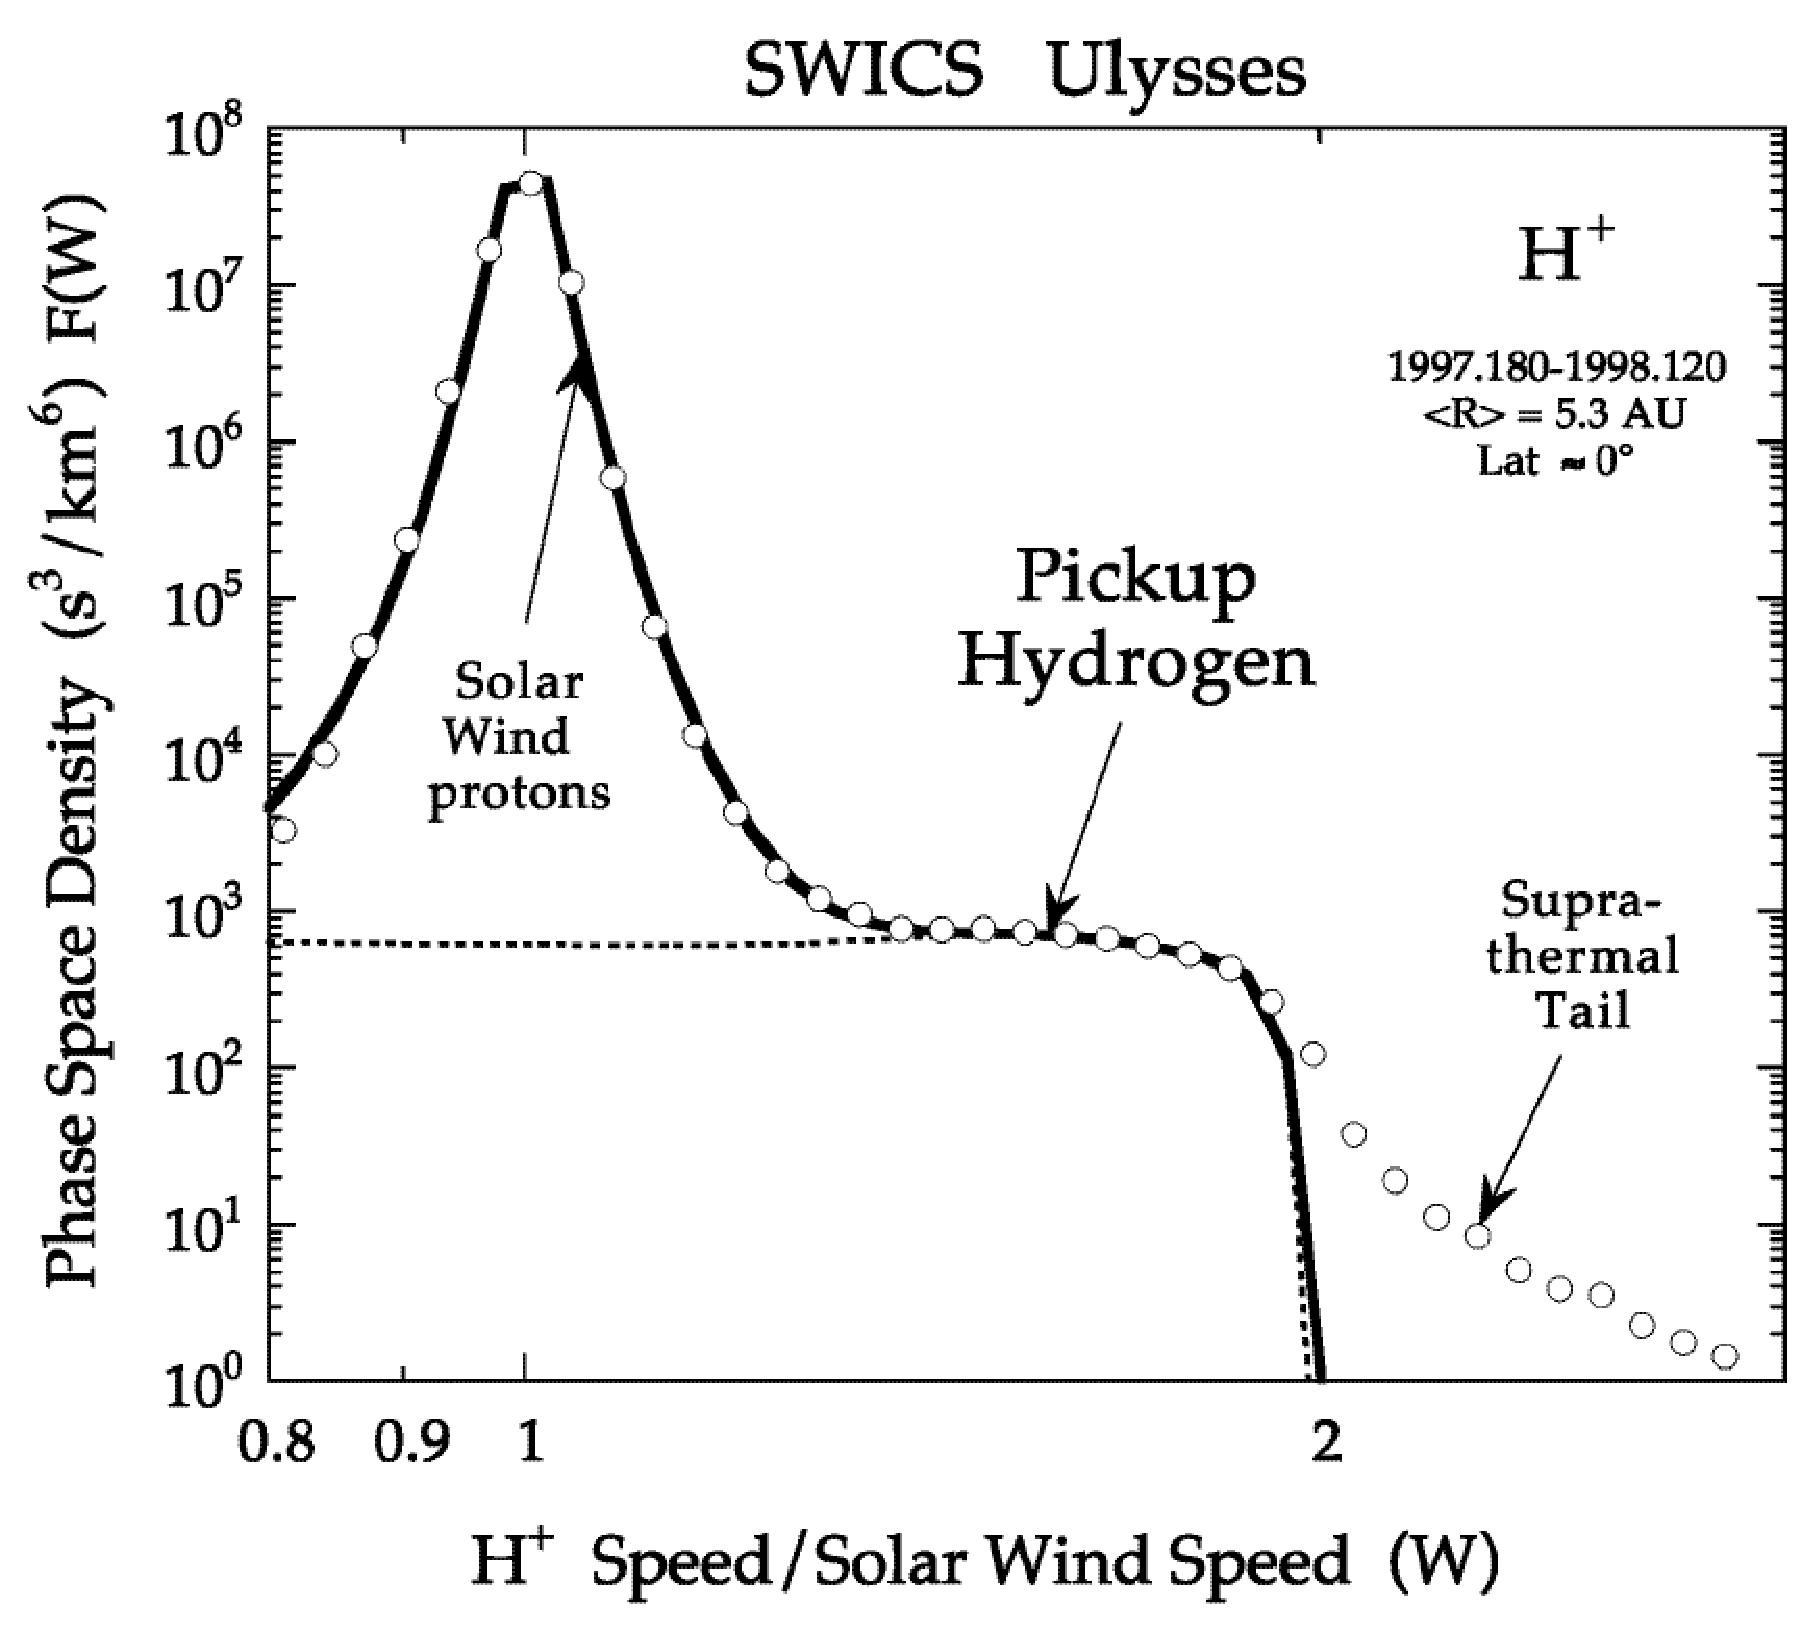
\includegraphics[width=.65\textwidth]{format/H_Distribution}
  \caption[Example of proton distributions for the quiet solar wind near 5 AU.]{Example of proton distributions for the quiet solar wind near 5 AU. Shown are the bulk distribution of the solar wind, the interstellar pickup ions that drop off at twice the solar wind speed, and the high-energy protons that make up the suprathermal tail. Figure from \citet{gloeckler01b}.}
  \label{fig:H_Distribution}
\end{figure}

\section{The Solar Wind}
\label{Solar Wind}

\subsection{Current Knowledge}
\label{SW Current Knowledge}
While he was not the first to postulate its existence, the physics of the solar wind was first explained by Eugene Parker in 1958 \citep{parker58}. Beginning with subsonic speeds close to the Sun, plasma accelerates away from the solar surface and reaches supersonic speeds in the corona. It continues to expand in a radial direction outward until it interacts with the material in interstellar space at the edge of the heliosphere, the Sun's sphere of influence. The wind draws the solar magnetic field along with it, creating spiral-shaped field lines as the Sun rotates \citep{parker59}. Mankind's understanding of the processes that govern the solar wind has increased as spacecraft have taken in situ measurements, but there are still some properties that remain unexplained, such as the precise origin of certain types of wind, as discussed below.

The solar wind travels a distance of one \ac{AU} before reaching Earth's orbit, where most of the current measurements have been taken (Table~\ref{tab:solar wind}). It is generally divided into two components, commonly referred to as the ``fast'' and ``slow'' solar wind. Originally, these terms were used to differentiate the wind by the speed with which it traveled, but more recent studies have shown that the two types of wind are more efficiently distinguished by their charge state composition (e.g., O$^{7+}$/O$^{6+}$) since the plasma can change speeds as it flows through space \citep{geiss95b, gloeckler03a}. Rather than the terms ``fast'' and ``slow'', more appropriate labels are descriptive of the wind's origin: ``coronal hole'' and ``streamer'' wind. These two types of wind are generated by different processes and have different compositions, temperatures, speeds, and origins.
\begin{table}[htbp]
	\centering
		\begin{tabular}{l|c|c}
		                                                               & Coronal Hole Wind & Streamer Wind     \\ \hline
      bulk speed \footnotesize{$\left(\text{km s}^{-1}\right)$}    & 750               & 400               \\ \hline
      thermal speed \footnotesize{$\left(\text{km s}^{-1}\right)$} & 32                & 35                \\ \hline
      H$^+$ density \footnotesize{$\left(\text{cm}^{-3}\right)$}   & 2.5               & 8.7               \\ \hline
      frozen-in temperature \footnotesize{$\left(\text{K}\right)$} & 8 x 10$^5$        & 1.4--1.6 x 10$^6$ \\ \hline

		\end{tabular}
	\caption[Average characteristics of the solar wind at 1 AU.]{Average characteristics of the solar wind at 1 AU. The temperature is derived from the freeze-in temperature of C$^{6+}$/C$^{5+}$, which freezes in near the solar wind source altitude. Data compiled from \citet{vonsteiger95, gloeckler98a, ipavich98, mccomas00, feldman05}.}
	\label{tab:solar wind}
\end{table}

As solar wind ions escape from the photosphere and travel up through the corona, they experience collisions with energetic electrons that ionize them to different degrees. As they travel farther through the corona, continuously accelerating, the density of coronal electrons decreases and the particles experience fewer collisions. When the timescale for ionization or recombination becomes longer than the timescale of the solar wind to expand through a density scale height, the charge state of the ion is said to be ``frozen in,'' branding the ion with the coronal region and electron temperature of its origin \citep{hundhausen68}. The streamer wind has a distinct characteristic of being enriched in elements with a low ($\le$ 10 eV) \ac{FIP} by a factor of 3--4 over the photospheric value. The coronal hole wind does not show this density enhancement, and measurements have revealed abundances of low-\ac{FIP} elements that match ratios in the photosphere \citep{vonsteiger93}. The streamer wind also has a higher and more variable freeze-in temperature than the coronal hole wind. One explanation for this describes solar plasma trapped and heated in large coronal loops that are eventually opened by interchange reconnection, releasing the plasma \citep{gosling95, fisk98, fisk99a}.

The coronal hole wind originates in the open flux regions of the Sun, which contain low-density plasma and concentrations of magnetic flux that are all the same polarity. During solar minimum these regions are clustered around the poles of the Sun, while during solar maximum they appear at all latitudes. Plasma in open flux regions is also released from flux loops, but the high concentration of open flux increases the probability that the loops will open before they can heat and fractionate the plasma. The anti-correlation between freeze-in temperature and solar wind speed shown in Table~\ref{tab:solar wind} can be interpreted in a simplistic way as a sign of different sized loops. The long-lived loops that produce the streamer wind will expand and rise slowly into the corona, where the temperatures are hotter, before being opened \citep{fisk98, fisk01a}. The short-lived loops that yield the coronal hole wind are opened while they are still small and close to the cooler surface \citep{fisk99a, fisk03, wimmer03b}.

 \chapter{Electronic Mechanism of H adsorptions on ZnO Surfaces}
 \label{chap:ZnO_H}
 \input{Chap1/chap1}
 
 \chapter{Alloy segregations in Ag grain boundaries}
 \label{chap:Ag_W}
 \input{Chap2/chap2}
 
 \chapter{Dopants in Mg to enhance its corrosion resistance}
 \label{chap:Mg_H}
 \input{Chap3/chap3}
 
 \chapter{Grand Canonical Monte Carlo simulations of Ag thin film depositions}
 \label{chap:Ag/ZnO}
 \input{Chap4/chap4}
 
 \chapter{Kinetic Monte Carlo simulations of Solute Clustering in multi-component Al alloys}
 \label{chap:Al/Vac}
 \input{Chap5/chap5}
 
 \chapter{Conclusion}
 \label{chap:Conc}
 \section{Summary}

Currently, to fulfill requirements of the quality and combination of different properties of materials, more costly and complicated processing techniques have to be used. However, for civilian-sector industrial-scale applications, cost and sustainability are also of vital importance. We need to find new strategies to reduce both the usage of costly processing facilities and the degradation of materials quality. In my dissertation, the thermodynamic driving force and key kinetic steps during relevant alloy processing procedures are studied systematically by theoretical/simulational tools at the atomistic scale. In Chapter \ref{chap:ZnO_H} and \ref{chap:Ag/ZnO}, efforts are made to improving the Ag thin-film quality during sputtering by changing substrate structures and chemistry. In Chapter \ref{chap:Mg_H}, we focus on the Mg alloy corrosion issue, and create a build-in corrosion-resistant mechanism. In Chapter \ref{chap:Al/Vac}, efforts are made to slow down cluster nucleation in Al alloy during natural aging in order to avoid costly hot-working, warm stamping procedures. The main conclusions include:

In Chapter \ref{chap:ZnO_H}, the thermodynamic driving force of H adsorption on anion-terminated (000$\overline{1}$) surfaces of pure and doped wurtzite ZnO are investigated under varying H surface coverage conditions. A $\frac{1}{2}$ \ac{ML} of adsorbed H changes the electronic structure of pure ZnO (000$\overline{1}$) surface from metallic to semiconductor state by saturating unpaired electrons of surface oxygen atoms. This closed-shell electron configuration of ZnO (000$\overline{1}$) surface significantly reduces the adsorption strengths of subsequent H atoms, making the dissociative adsorption of a hydrogen molecule endothermic. A simple electron counting model is applied to predict and tune the coverage-dependent H adsorption strengths on semiconductor surfaces. When doping elements (such as Al, Ti, and V) have more valence electrons than Zn, the critical H coverage will decrease to lower coverages. We also expand the method of tuning H equilibrium coverage to other similar polar semiconductors, such as wurtzite GaN (000$\overline{1}$), and zincblende ZnS ($\overline{1}$$\overline{1}$$\overline{1}$) surfaces. This method provides a general way to generate desired surface reconstructions of dielectric substrates before sputtering.

In Chapter \ref{chap:Ag/ZnO}, we utilize \ac{GCMC} simulation to understand the reason why ZnO is the best substrate option for Ag thin film deposition. The hexagonal substrate, like ZnO (000$\overline{1}$), are robust to lattice constant and bonding strength changes and yields most \{111\} orientation Ag thin films. Besides, to achieve more continuous Ag thin films with less use of Ag, elements, like Pd, Sb, Se, Sn, and Te, can be added as ``anchor'' sites to incoming Ag atoms. With 0.05\ac{ML} of ``anchor'' sites on the substrate, more nuclei can be achieved. We also search for alloying elements that can segregate in Ag grain boundaries to stabilize grain size during heat treatments. \ac{DFT} calculation shows that tungsten (W) does not segregation in Ag grain boundaries, which is inconsistent with experiments. We suspect that alloying elements can not only change the chemistry of the grain boundaries but also disrupt the atomistic structure of grain boundaries in alloys.

In Chapter \ref{chap:Mg_H}, our computational procedure predicts that six p-block elements meet thermodynamic stability and H adsorption criteria, and they rank according to their ability to reduce H adsorption energies and the \ac{HER} rate as follows: $\text{As} > \text{Ge} > \text{Si} > \text{Ga} > \text{P} \approx \text{Al}$. Results for As, the most effective corrosion-inhibiting element, and Ge are in qualitative accord with recent experiments. While none of the 68 elements was found to enhance H adsorption, the six p-block elements reduce H adsorption via strong orbital overlap (Pauli repulsion) between their outer-shell orbitals and the s orbitals of H adsorbates. We also extend our model to other major precipitates in Mg alloy. This chapter solves the problem of applying My alloys to the civilian-sector industry by improving the sustainability of alloys.

In Chapter \ref{chap:Al/Vac}, we first demonstrate that the \acf{BEP} relationship fails to provide quantitatively accurate diffusion barriers for multi-component alloys. Then we develope a \ac{NN} model to predict diffusion barriers using thousands of \ac{DFT} calculated barriers. And a \ac{kMC} method based on this \ac{NN} model is used to study the early transition behavior from a supersaturated solid solution to \ac{GP} zone of Al 7000 series alloys. A local super-basin method together with \ac{LRU} cache is also implemented to accelerate \ac{kMC} simulations. Following our general strategy to add a trace amount of element, we study the effect of adding pseudo-atoms with different ability to change vacancy diffusion barriers. At last, we compare current methods to evaluate the strengthening effect of precipitates and propose potential machine learning methods based on cluster geometry and chemical information. Quantitative analysis methods to describe the chemical and structural properties of clusters are developed, which could be used as inputs to predict precipitate strengthening effects.



\section{Future Work}

First, in Chapter \ref{chap:Mg_H}, we discuss the possibility of using six p-elements to ``poisson'' Fe precipitates surfaces of Mg alloys. However, the top two most efficient elements are As and Ge. Even though they will achieve the best effects, As is toxic and Ge is still relatively expensive. It will be worthwhile to explore the combination of two alternative elements that can achieve a similar effect.

Second, efforts are made, in Section \ref{Chap:Ag/ZnO:GB}, to search for potential elements that can stabilize Ag grain boundaries. Traditionally, the theoretical approach to study the alloy segregation effects is firstly obtained relaxed grain boundary structures from pure metals and then substitute dilute atoms to calculate alloy segregation energies. One possibility of the discrepancy we observed could be that alloying elements can not only change the chemistry of the grain boundaries but also change the atomistic structure of grain boundaries in alloys. Besides, in reality, more complicated grain boundaries, like grain boundary complexions, exist. \cite{cantwell2014grain} Therefore, more complicated grain boundary structures need to be obtained by global optimization methods, e.g. evolutionary algorithm, to investigate the alloy segregation effects.

Third, in Section \ref{Chap:Al/Vac:section:KMC}, different approaches, such as \ac{LRU} cache, \ac{LSKMC}, parallel computing, are implemented to speed up the simulation for a longer time domain. So far, the simulated time span can be achieved is still at the level between $\sim$seconds to $\sim$minutes. This is still not fast enough to simulate the entire process of the \ac{GP} zone clustering. This further speedup can be achieved by:

\begin{enumerate}

  \item One of the speed limitations of our current model lies in the complexity of our \ac{NN} architecture. If a smaller architecture with fewer weight parameters can be achieved, then during the serving stage each prediction step will be more efficient.

  \item Our program is written in C++ with pure \ac{MPI}, which means one \ac{MPI} process on each core. The optimal efficiency can be achieved by using $12*N$ cores, where $N$ is the number of vacancies in the configuration. In this parallel schema, one process(core) takes care of one possible jumping event, respectively. To speed up, we can combine \ac{MPI} with OpenMP. OpenMP is a shared memory multiprocessing library. In this hybrid schema, we can use $12*N*M$, where $M$ is the number of threads per core. Then one event can be calculated by $M$ threads.

  \item \ac{LRU} cache exhibits a great speed up by looking up existing keys of encoding swiftly. However, it only works in a serial version for now. One problem needs to be solved before multi-core \ac{LRU} cache can be implemented. The problem lies in different cores do not share the same memory. Thus each core can only store one specific event out of the 12 possible events. In the consecutive iterations, the probability of a core encounter with the same event is largely reduced. Thus the time of executing one step will be determined by the slowest one. One strategy is to transfer several most recent data across the cores once several steps. In this way, all the cores will cover all the 12 possible events of recent steps.

\end{enumerate}

Fourth, we would like to continue to investigate the intrinsic mechanisms of GP zone clusters nucleation and growth kinetics. Although the sensitivity tests in Chapter \ref{Chap:Al/Vac:pseudo} could yield qualitatively results for the effect of pseudo atoms, to match such an element will still take more time and computational resources. And a surrogate model based on chemical, structural, and energetical properties of the cluster to predict strengthening effects still need to be developed.

Fifth, the \ac{kMC} simulation in this thesis ignores the effect of strain introduced by clustering or alloying, and only consider vacancy diffusions of an on-lattice manner. The effects of the distribution of solute atoms on the strain field and interaction between strain effects and dislocations still remain unknown. The strain effect can be implemented by using regular on-lattice \ac{kMC} with a continuum analytical function for the strain energetic contribution. The strain offsets could depend on the local concentration of the simulation cell and the concentration of the simulation cell would be flexible and interchangeable with the universe using a grand canonical ensemble mentioned in Section \ref{Chap:Mech:GCMC}.

Sixth, details about how clustering in Al alloy increases strength is still unclear. In previous studies, either only elastic strain effects are considered \cite{zhao2014cluster} or the strain effects and chemical effects were considered and estimated separately \cite{yasi2010first}. The elastic strain effects and chemical effects could couple together and become more complicated when the chemical composition of clusters becomes complex. In order to better understand their effects on strengthening, we propose to use advanced machine learning models to predict the strengthening effects. Output parameters and cluster atomic structures from Chapter \ref{chap:Al/Vac}, such as chemical composition, cluster size distributions, and bond statistics will be the input parameters of the classical continuum model or machine learning surrogate model to predict the hardness change during natural aging. If we assume that the effects of trace solute elements and heat treatment procedures on natural aging hardening can be fully described by the structural, mechanical and energetics parameters generated in the above \ac{kMC} simulations. Then we can build similar surrogate models to predict the natural aging hardening effects under the influence of various types of solute elements.

Based on the previous point, the effect of chemical bonding is more complicated than the strain effects and it will need detailed electronic structure investigation using first-principles calculations. In the very latest research, Liu et al. \cite{liu2020formation} found that at room temperature, \ac{GP} II zone clusters in Al-Zn-Mg alloys form very slowly. It will take a couple of weeks for the growth of \ac{GP} zone clusters. However, the hardness of Al-Zn-Mg alloys still increases very quickly during natural aging. The authors claim that solute cluster hardening is accountable for the rapidly hardening effect of the alloy. When dislocations cut through an ordered solute cluster, only local bond changes will be observed. Additional energy is required to create an anti-phase boundary (APB). Hence under quasi-equilibrium thermodynamics, the energy differences between these initial and final structures might be responsible for the hardening effect. It is then critical to figure out how the short-range orderliness of clusters will affect the hardness. Besides, as the size of the solute cluster increases, dislocation cutting through precipitates becomes more difficult. On the other hand, dislocations prefer to bend around the particle by Orowan Looping. Therefore, the optimal cluster size distribution might also be of interest in future work. 
 
\startappendices
 \appendix{blah blah blah}
 \label{app:CN Scheme}
 For the diffusion process, The equation was solved using a two-dimensional implicit Crank-Nicolson scheme, which is unconditionally stable and second-order accurate in both time and space \citep{crank47}. In the conventional notation, the two-dimensional numerical scheme using central differencing can be written for a uniform Cartesian grid as 
\begin{eqnarray}
\nonumber\left(1+2\mu\right)u^{t+1}_{i,j}-\frac{\mu}{2}\left(u^{t+1}_{i+1,j}+u^{t+1}_{i-1,j}+u^{t+1}_{i,j+1}+u^{t+1}_{i,j-1}\right)\\
=\left(1-2\mu\right)u^{t}_{i,j}+\frac{\mu}{2}\left(u^{t}_{i+1,j}+u^{t}_{i-1,j}+u^{t}_{i,j+1}+u^{t}_{i,j-1}\right),
\end{eqnarray}

\noindent where $u^{t}_{i,j}$ is the value of the parameter undergoing the diffusion ($B_{r}$ in this case) at position $(i, j)$ at time \textit{t}. The von Neumann number on a uniform grid is $\mu=\xi{\Delta}t/\left({\Delta}x\right)^{2}$, where the size of the grid square is $\Delta x$ on each side, and the diffusion coefficient $\xi$ describes the speed at which the mathematical diffusion takes place. When deriving the two-dimensional Crank-Nicolson scheme in spherical coordinates, the von Neumann number is written as $\mu=\xi{\Delta}t/\left(r\Delta\theta\right)^{2}$, where $\Delta\theta=\Delta\phi$, and the cosine is replaced by the central difference of the sine to remain consistent with the discrete nature of the other terms. Care must be taken at the poles, where the central differencing is replaced by forward or backward differencing. To keep second-order accuracy with forward or backward differencing, the series must be carried out to higher-order terms in the derivation. The two-dimensional numerical scheme using central differencing can be written for a uniform spherical grid as
\begin{multline}
\left(1+\mu+\frac{\mu}{\sin^{2}\theta_{i,j}}\right)u^{t+1}_{i,j}-\frac{\mu}{2}\left[1+\frac{\left(\sin\theta_{i+1,j}-\sin\theta_{i-1,j}\right)}{4\sin\theta_{i,j}}\right]u^{t+1}_{i+1,j}\\
 -\frac{\mu}{2}\left[1-\frac{\left(\sin\theta_{i+1,j}-\sin\theta_{i-1,j}\right)}{4\sin\theta_{i,j}}\right]u^{t+1}_{i-1,j}-\frac{\mu}{2}\frac{1}{\sin^{2}\theta_{i,j}}u^{t+1}_{i,j+1}-\frac{\mu}{2}\frac{1}{\sin^{2}\theta_{i,j}}u^{t+1}_{i,j-1}\\
 =\left(1-\mu-\frac{\mu}{\sin^{2}\theta_{i,j}}\right)u^{t+1}_{i,j}+\frac{\mu}{2}\left[1+\frac{\left(\sin\theta_{i+1,j}-\sin\theta_{i-1,j}\right)}{4\sin\theta_{i,j}}\right]u^{t+1}_{i+1,j}\\
 +\frac{\mu}{2}\left[1-\frac{\left(\sin\theta_{i+1,j}-\sin\theta_{i-1,j}\right)}{4\sin\theta_{i,j}}\right]u^{t+1}_{i-1,j}+\frac{\mu}{2}\frac{1}{\sin^{2}\theta_{i,j}}u^{t+1}_{i,j+1}+\frac{\mu}{2}\frac{1}{\sin^{2}\theta_{i,j}}u^{t+1}_{i,j-1}.
 \label{CN Spherical}
\end{multline}

Although it is unconditionally stable, a marching scheme such as this will depend on the value of $\mu$ for its accuracy. A lower choice of $\mu$ will lead to a more accurate solution at the expense of computational resources (i.e., a smaller time step ${\Delta}t$), while a higher value of $\mu$ will arrive at a solution more rapidly but with less accuracy (a larger time step). In this model, the value of the coefficient $\xi$ describes the speed of the mathematical relaxation and, since it does not describe a physical process, can be chosen arbitrarily. Thus the only restriction for this scheme will lie in keeping $\mu$ small for accuracy and assigning either $\xi$ or ${\Delta}t$. It can be seen that when $\mu$ is held constant, any choice for either $\xi$ or ${\Delta}t$ will lead to the same solution. A value of $\mu=1/4$ was chosen, with an arbitrary time step of ${\Delta}t=0.1$ s, and studied several different grid resolutions, with a grid size of 2.5$^\circ$ x 2.5$^\circ$ (72 x 144 grid spaces) on a uniform spherical grid used for the comparisons in this paper. The relaxation was allowed to continue on a sphere of $r=R_{\sun}$ until the difference in magnetic field magnitude between any cell and its neighbor was of order $10^{-1}{\mu}T$.
 
\startbibliography
 \begin{singlespace} % Bibliography must be single spaced
  \bibliography{References}   % Use the BibTeX file ``References.bib''.
 \end{singlespace}

% An external Abstract that can be printed at the end of the document, 
% for separate submission to Rackham. Comment it out when not needed. - jg
%\startextabstractpage
%{The Title of Your Dissertation}{Your Name}{Chair: Albert Einstein}
%In my dissertation, the thermodynamic driving forces and kinetics of critical reaction steps during advanced alloy processing are studied systematically by theoretical models and simulation tools at the atomistic scale. These efforts include improving the Ag thin-film quality during sputtering, discovering a build-in corrosion-resistant mechanism for cast Mg alloys, and slowing down cluster nucleation and growth in Al solid solution alloys during natural aging to avoid costly hot stamping procedures. First, the thermodynamic driving force of H adsorption on anion-terminated (000$\overline{1}$) surfaces of pure and doped wurtzite ZnO as dielectric substrates are investigated under varying H surface coverage conditions. Understanding of these H adsorption mechanisms provides a general way to design substrate surfaces with desired binding strengths for the Ag thin-film. Second, \acf{GCMC} simulations are conducted to simulate the deposition "kinetics" of Ag thin film on substrates, which can be constructed based on the structures and properties of H-adsorbed ZnO (000$\overline{1}$) surfaces. The results demonstrate the reason why ZnO is the most suitable substrate for Ag thin film deposition and the mechanism to achieve thinner continuous Ag films by adding "anchor'' sites on the substrate surface. We use first-principles calculations to search for potential dopant elements as good "anchor'' sites on ZnO substrates and other dopants to stabilize the Ag grain boundaries to improve the polycrystalline Ag thin-film during heat treatment. Third, the \acf{HER} as the cathodic reaction on surfaces of the second-phase transition-metal (Fe) particles can speed up the corrosion of cast Mg metals and alloy. Thus, thermodynamic criteria to slow down the HER are used for high-throughput first-principles computations to search alloying elements that can reduce HER rate to achieve build-in corrosion resistance for cast Mg alloys. Our first-principles search goes across the periodic table and discovers six p-block elements that can increase the corrosion resistance for Mg, consistent with the available experimental results. Fourth, \acf{kMC} simulations are performed to study the early transition behavior from a supersaturated solid solution to \acf{GP} zone of Al 7000 series alloys at room temperature (so-called natural aging), which is critical for their thermal-mechanical processing in automobile manufacturing. Our kMC method include a \acf{NN} model trained by thousands of \ac{DFT} calculations to accurately predict vacancy migration barriers in Al-Mg-Zn-based alloys. Besides, advanced modeling approaches like \acf{LRU} cache and \acf{LSKMC} are also implemented to speed up the kMC simulations in order to directly study the natural aging of Al alloys in the realistic time scales.
%\label{ExtAbstract}

\end{document}